\documentclass[10pt,a4paper]{article}

\usepackage[T1]{fontenc}
\usepackage[utf8]{inputenc}
\usepackage[english]{babel}
\usepackage[sc]{mathpazo}
\usepackage{microtype}
\usepackage[a4paper,margin=2.1cm,top=1.9cm,bottom=1.9cm]{geometry}
\usepackage{amsmath,amssymb}
\usepackage{graphicx}
\usepackage{booktabs,tabularx,makecell}
\usepackage{enumitem}
\usepackage[font=small,labelfont=bf,labelsep=colon,skip=3pt]{caption}
\usepackage{xcolor}
\usepackage[most]{tcolorbox}
\usepackage[hidelinks]{hyperref}
\usepackage{float}
\usepackage{url}
\usepackage{tikz}

\definecolor{blueI}{HTML}{2A78D6}
\definecolor{orangeJ}{HTML}{EB6834}
\definecolor{ink}{HTML}{52514E}
\newtcolorbox{summary}{enhanced, breakable, colback=blueI!5!white, colframe=blueI, boxrule=0pt,
  leftrule=2.4pt, arc=0pt, outer arc=0pt, left=6pt, right=6pt, top=3pt, bottom=3pt}
\newtcolorbox{reading}{enhanced, breakable, colback=black!3!white, colframe=black!45, boxrule=0pt,
  leftrule=1.6pt, arc=0pt, outer arc=0pt, left=5pt, right=5pt, top=2pt, bottom=2pt, fontupper=\small}

\graphicspath{{../out/d120_eh500_ez300_th45_g120_q0.1/}{../../../../ideas/group-identification/figures/}}
\newcommand{\G}{\mathrm{G}}
\newcommand{\A}{\mathrm{A}}
\newcommand{\Sl}{\mathrm{S}}
\setlist{itemsep=1pt, topsep=2pt, parsep=0pt, leftmargin=1.3em}
\setlength{\parindent}{0pt}
\setlength{\parskip}{3pt}
\captionsetup{font=footnotesize}
\newcommand{\Abreast}{35}
\newcommand{\AtDeparture}{1\,179}
\newcommand{\AtLanding}{1\,358}
\newcommand{\ClimbA}{29.1}
\newcommand{\ClimbG}{33.0}
\newcommand{\ClimbS}{30.8}
\newcommand{\DClimbFlight}{$+$5.71}
\newcommand{\DClimbFlightBand}{[$+$5.52, $+$5.92]}
\newcommand{\DClimbGroupSdh}{$+$3.28}
\newcommand{\DClimbGroupSdhBand}{[$+$3.11, $+$3.47]}
\newcommand{\DClimbRaw}{$+$2.20}
\newcommand{\DClimbRawBand}{[$+$1.96, $+$2.45]}
\newcommand{\DClimbSdh}{$+$3.43}
\newcommand{\DClimbSdhBand}{[$+$3.19, $+$3.63]}
\newcommand{\DClimbSel}{$+$0.43}
\newcommand{\DClimbSelBand}{[$+$0.25, $+$0.59]}
\newcommand{\DClimbSizeMax}{$+$4.0}
\newcommand{\DClimbSizeMin}{$+$2.0}
\newcommand{\DCompClimb}{$-$1.23}
\newcommand{\DCompFound}{$+$2.06}
\newcommand{\DCompHlocHundred}{$+$0.006}
\newcommand{\DCompHlocThousand}{$+$0.014}
\newcommand{\DCompRate}{$+$0.009}
\newcommand{\DCompSink}{$-$8.6}
\newcommand{\DCompSpeed}{$+$1.20}
\newcommand{\DCompXc}{$+$0.55}
\newcommand{\DFoundFlight}{$+$8.75}
\newcommand{\DFoundFlightBand}{[$+$8.37, $+$9.15]}
\newcommand{\DFoundGroupSdh}{$+$2.59}
\newcommand{\DFoundGroupSdhBand}{[$+$2.25, $+$2.99]}
\newcommand{\DFoundRaw}{$+$6.18}
\newcommand{\DFoundRawBand}{[$+$5.82, $+$6.46]}
\newcommand{\DFoundSdh}{$+$4.12}
\newcommand{\DFoundSdhBand}{[$+$3.68, $+$4.54]}
\newcommand{\DFoundSel}{$+$1.60}
\newcommand{\DFoundSelBand}{[$+$1.23, $+$1.97]}
\newcommand{\DHlocHundredFlight}{$-$0.009}
\newcommand{\DHlocHundredFlightBand}{[$-$0.009, $-$0.008]}
\newcommand{\DHlocHundredGroupSdh}{$+$0.002}
\newcommand{\DHlocHundredGroupSdhBand}{[$+$0.001, $+$0.002]}
\newcommand{\DHlocHundredRaw}{$+$0.008}
\newcommand{\DHlocHundredRawBand}{[$+$0.007, $+$0.009]}
\newcommand{\DHlocHundredSdh}{$+$0.002}
\newcommand{\DHlocHundredSdhBand}{[$+$0.001, $+$0.003]}
\newcommand{\DHlocHundredSel}{$+$0.005}
\newcommand{\DHlocHundredSelBand}{[$+$0.004, $+$0.005]}
\newcommand{\DHlocThousandFlight}{$+$0.037}
\newcommand{\DHlocThousandFlightBand}{[$+$0.035, $+$0.039]}
\newcommand{\DHlocThousandFlightSeven}{$+$0.087}
\newcommand{\DHlocThousandFlightSevenBand}{[$+$0.069, $+$0.105]}
\newcommand{\DHlocThousandFlightTwo}{$+$0.026}
\newcommand{\DHlocThousandFlightTwoBand}{[$+$0.023, $+$0.029]}
\newcommand{\DHlocThousandGroupSdh}{$+$0.043}
\newcommand{\DHlocThousandGroupSdhBand}{[$+$0.040, $+$0.046]}
\newcommand{\DHlocThousandMiddleMax}{$+$0.004}
\newcommand{\DHlocThousandMiddleMin}{$-$0.015}
\newcommand{\DHlocThousandRaw}{$+$0.055}
\newcommand{\DHlocThousandRawBand}{[$+$0.053, $+$0.057]}
\newcommand{\DHlocThousandSdh}{$+$0.041}
\newcommand{\DHlocThousandSdhBand}{[$+$0.038, $+$0.044]}
\newcommand{\DHlocThousandSel}{$+$0.003}
\newcommand{\DHlocThousandSelBand}{[$+$0.001, $+$0.006]}
\newcommand{\DHlocThousandSevenTwoSdh}{$+$0.064}
\newcommand{\DHlocThousandSevenTwoSdhBand}{[$+$0.045, $+$0.085]}
\newcommand{\DRateFlight}{$+$0.024}
\newcommand{\DRateFlightBand}{[$+$0.019, $+$0.031]}
\newcommand{\DRateGroupSdh}{$+$0.029}
\newcommand{\DRateGroupSdhBand}{[$+$0.025, $+$0.034]}
\newcommand{\DRateRaw}{$+$0.040}
\newcommand{\DRateRawBand}{[$+$0.030, $+$0.051]}
\newcommand{\DRateSdh}{$+$0.031}
\newcommand{\DRateSdhBand}{[$+$0.025, $+$0.039]}
\newcommand{\DRateSel}{$+$0.007}
\newcommand{\DRateSelBand}{[$+$0.001, $+$0.012]}
\newcommand{\DSinkFlight}{$-$21.1}
\newcommand{\DSinkFlightBand}{[$-$22.1, $-$20.1]}
\newcommand{\DSinkFlightSeven}{$-$28.1}
\newcommand{\DSinkFlightTwo}{$-$17.6}
\newcommand{\DSinkGroupSdh}{$-$9.5}
\newcommand{\DSinkGroupSdhBand}{[$-$10.5, $-$8.6]}
\newcommand{\DSinkRaw}{$-$18.6}
\newcommand{\DSinkRawBand}{[$-$19.3, $-$17.8]}
\newcommand{\DSinkSdh}{$-$10.0}
\newcommand{\DSinkSdhBand}{[$-$10.7, $-$9.1]}
\newcommand{\DSinkSel}{$-$0.5}
\newcommand{\DSinkSelBand}{[$-$1.1, $+$0.3]}
\newcommand{\DSinkSevenTwoSdh}{$-$7.5}
\newcommand{\DSinkSevenTwoSdhBand}{[$-$11.8, $-$3.8]}
\newcommand{\DSinkSizeMax}{$-$9}
\newcommand{\DSinkSizeMin}{$-$3}
\newcommand{\DSpeedFlight}{$+$1.36}
\newcommand{\DSpeedFlightBand}{[$+$1.27, $+$1.46]}
\newcommand{\DSpeedGroupSdh}{$+$0.87}
\newcommand{\DSpeedGroupSdhBand}{[$+$0.79, $+$0.98]}
\newcommand{\DSpeedRaw}{$+$3.18}
\newcommand{\DSpeedRawBand}{[$+$2.97, $+$3.39]}
\newcommand{\DSpeedSdh}{$+$1.97}
\newcommand{\DSpeedSdhBand}{[$+$1.82, $+$2.10]}
\newcommand{\DSpeedSel}{$+$1.15}
\newcommand{\DSpeedSelBand}{[$+$1.05, $+$1.27]}
\newcommand{\DXcFlight}{$+$0.70}
\newcommand{\DXcFlightBand}{[$+$0.60, $+$0.78]}
\newcommand{\DXcGroupSdh}{$+$1.29}
\newcommand{\DXcGroupSdhBand}{[$+$1.16, $+$1.41]}
\newcommand{\DXcRaw}{$+$2.81}
\newcommand{\DXcRawBand}{[$+$2.59, $+$3.01]}
\newcommand{\DXcSdh}{$+$2.25}
\newcommand{\DXcSdhBand}{[$+$2.09, $+$2.39]}
\newcommand{\DXcSel}{$+$1.31}
\newcommand{\DXcSelBand}{[$+$1.21, $+$1.43]}
\newcommand{\DXcSevenTwoSdh}{$+$7.0}
\newcommand{\DXcSevenTwoSdhBand}{[$+$4.8, $+$8.7]}
\newcommand{\DelayMedian}{20}
\newcommand{\DelayNinety}{70}
\newcommand{\Entries}{31\,381}
\newcommand{\EntriesEarly}{34}
\newcommand{\Exits}{31\,202}
\newcommand{\FoundA}{45.9}
\newcommand{\FoundG}{49.5}
\newcommand{\FoundS}{43.3}
\newcommand{\GroupShareEvening}{22}
\newcommand{\GroupShareMorning}{38}
\newcommand{\GroupShareNoon}{52}
\newcommand{\GroupShareNoonHour}{12}
\newcommand{\HA}{0.914}
\newcommand{\HG}{0.916}
\newcommand{\HS}{0.899}
\newcommand{\HabitualDispersion}{2.73}
\newcommand{\HabitualExtreme}{12}
\newcommand{\HabitualExtremeNull}{3}
\newcommand{\HabitualNull}{1.00}
\newcommand{\HabitualNullHigh}{1.07}
\newcommand{\HabitualPilots}{946}
\newcommand{\HabitualRoles}{22\,231}
\newcommand{\HlocHundredA}{0.932}
\newcommand{\HlocHundredG}{0.927}
\newcommand{\HlocHundredS}{0.919}
\newcommand{\HlocThousandA}{0.860}
\newcommand{\HlocThousandAloneMax}{0.871}
\newcommand{\HlocThousandAloneMin}{0.861}
\newcommand{\HlocThousandG}{0.893}
\newcommand{\HlocThousandS}{0.837}
\newcommand{\HlocThousandSeven}{0.944}
\newcommand{\HlocThousandTwo}{0.889}
\newcommand{\LeadClimb}{$+$0.91 [$+$0.57, $+$1.25]}
\newcommand{\LeadFound}{$-$0.01 [$-$1.03, $+$0.83]}
\newcommand{\LeadHlocHundred}{$-$0.002 [$-$0.002, $-$0.001]}
\newcommand{\LeadHlocThousand}{$-$0.003 [$-$0.004, $-$0.001]}
\newcommand{\LeadRate}{$+$0.021 [$+$0.014, $+$0.028]}
\newcommand{\LeadSink}{$+$1.6 [$-$0.9, $+$4.5]}
\newcommand{\LeadSpeed}{$+$0.86 [$+$0.74, $+$0.99]}
\newcommand{\PPAfterBeforeClimb}{$-$1.4}
\newcommand{\PPAfterBeforeDH}{$+$0.004}
\newcommand{\PPAfterBeforeDHBand}{[$+$0.003, $+$0.005]}
\newcommand{\PPAfterBeforeDHloc}{$-$0.003}
\newcommand{\PPAfterBeforeDHlocBand}{[$-$0.007, $+$0.001]}
\newcommand{\PPAfterBeforeDHlocHundred}{$+$0.006}
\newcommand{\PPAfterBeforeEvents}{6\,320}
\newcommand{\PPAfterBeforeFound}{$-$2.8}
\newcommand{\PPAfterBeforeRate}{$+$0.043}
\newcommand{\PPAfterBeforeSink}{$+$9.1}
\newcommand{\PPAfterBeforeSpeed}{$+$0.33}
\newcommand{\PPCtrlAClimb}{$-$1.1}
\newcommand{\PPCtrlADH}{$+$0.005}
\newcommand{\PPCtrlADHBand}{[$+$0.004, $+$0.005]}
\newcommand{\PPCtrlADHloc}{$-$0.002}
\newcommand{\PPCtrlADHlocBand}{[$-$0.005, $+$0.000]}
\newcommand{\PPCtrlADHlocHundred}{$+$0.005}
\newcommand{\PPCtrlAEvents}{16\,998}
\newcommand{\PPCtrlAFound}{$-$1.4}
\newcommand{\PPCtrlARate}{$+$0.018}
\newcommand{\PPCtrlASink}{$+$3.3}
\newcommand{\PPCtrlASpeed}{$+$0.07}
\newcommand{\PPCtrlSClimb}{$-$1.6}
\newcommand{\PPCtrlSDH}{$+$0.009}
\newcommand{\PPCtrlSDHBand}{[$+$0.008, $+$0.009]}
\newcommand{\PPCtrlSDHloc}{$-$0.002}
\newcommand{\PPCtrlSDHlocBand}{[$-$0.003, $-$0.000]}
\newcommand{\PPCtrlSDHlocHundred}{$+$0.010}
\newcommand{\PPCtrlSEvents}{69\,648}
\newcommand{\PPCtrlSFound}{$-$2.3}
\newcommand{\PPCtrlSRate}{$+$0.011}
\newcommand{\PPCtrlSSink}{$+$4.9}
\newcommand{\PPCtrlSSpeed}{$+$0.04}
\newcommand{\PPEntryClimb}{$+$0.7}
\newcommand{\PPEntryDH}{$+$0.010}
\newcommand{\PPEntryDHBand}{[$+$0.009, $+$0.011]}
\newcommand{\PPEntryDHloc}{$+$0.027}
\newcommand{\PPEntryDHlocBand}{[$+$0.023, $+$0.031]}
\newcommand{\PPEntryDHlocHundred}{$+$0.005}
\newcommand{\PPEntryEvents}{6\,524}
\newcommand{\PPEntryFound}{$+$0.0}
\newcommand{\PPEntryRate}{$+$0.046}
\newcommand{\PPEntrySink}{$-$2.3}
\newcommand{\PPEntrySpeed}{$+$0.92}
\newcommand{\PPExitClimb}{$+$1.5}
\newcommand{\PPExitDH}{$+$0.005}
\newcommand{\PPExitDHBand}{[$+$0.004, $+$0.006]}
\newcommand{\PPExitDHloc}{$+$0.031}
\newcommand{\PPExitDHlocBand}{[$+$0.028, $+$0.033]}
\newcommand{\PPExitDHlocHundred}{$-$0.001}
\newcommand{\PPExitEvents}{13\,643}
\newcommand{\PPExitFound}{$+$1.2}
\newcommand{\PPExitRate}{$-$0.007}
\newcommand{\PPExitSink}{$-$10.9}
\newcommand{\PPExitSpeed}{$+$0.52}
\newcommand{\PPProfileEvents}{3\,334}
\newcommand{\PPProfileHEnd}{0.931}
\newcommand{\PPProfileHPost}{0.925}
\newcommand{\PPProfileHPre}{0.920}
\newcommand{\PPProfileHStart}{0.931}
\newcommand{\PPProfileHlocEnd}{0.911}
\newcommand{\PPProfileHlocHundredEnd}{0.942}
\newcommand{\PPProfileHlocHundredPost}{0.942}
\newcommand{\PPProfileHlocHundredPre}{0.935}
\newcommand{\PPProfileHlocHundredStart}{0.940}
\newcommand{\PPProfileHlocPost}{0.876}
\newcommand{\PPProfileHlocPre}{0.879}
\newcommand{\PPProfileHlocStart}{0.910}
\newcommand{\PPShortAfterBeforeClimb}{$-$1.5}
\newcommand{\PPShortAfterBeforeDH}{$+$0.004}
\newcommand{\PPShortAfterBeforeDHBand}{[$+$0.003, $+$0.005]}
\newcommand{\PPShortAfterBeforeDHloc}{$+$0.002}
\newcommand{\PPShortAfterBeforeDHlocBand}{[$-$0.001, $+$0.006]}
\newcommand{\PPShortAfterBeforeDHlocHundred}{$+$0.006}
\newcommand{\PPShortAfterBeforeEvents}{14\,482}
\newcommand{\PPShortAfterBeforeFound}{$-$4.1}
\newcommand{\PPShortAfterBeforeRate}{$+$0.017}
\newcommand{\PPShortAfterBeforeSink}{$+$9.6}
\newcommand{\PPShortAfterBeforeSpeed}{$+$0.17}
\newcommand{\PPShortCtrlAClimb}{$-$2.1}
\newcommand{\PPShortCtrlADH}{$+$0.006}
\newcommand{\PPShortCtrlADHBand}{[$+$0.005, $+$0.006]}
\newcommand{\PPShortCtrlADHloc}{$-$0.011}
\newcommand{\PPShortCtrlADHlocBand}{[$-$0.015, $-$0.008]}
\newcommand{\PPShortCtrlADHlocHundred}{$+$0.006}
\newcommand{\PPShortCtrlAEvents}{33\,658}
\newcommand{\PPShortCtrlAFound}{$-$2.8}
\newcommand{\PPShortCtrlARate}{$-$0.001}
\newcommand{\PPShortCtrlASink}{$+$3.4}
\newcommand{\PPShortCtrlASpeed}{$-$0.29}
\newcommand{\PPShortCtrlSClimb}{$-$2.0}
\newcommand{\PPShortCtrlSDH}{$+$0.009}
\newcommand{\PPShortCtrlSDHBand}{[$+$0.009, $+$0.010]}
\newcommand{\PPShortCtrlSDHloc}{$-$0.007}
\newcommand{\PPShortCtrlSDHlocBand}{[$-$0.008, $-$0.005]}
\newcommand{\PPShortCtrlSDHlocHundred}{$+$0.010}
\newcommand{\PPShortCtrlSEvents}{107\,324}
\newcommand{\PPShortCtrlSFound}{$-$3.0}
\newcommand{\PPShortCtrlSRate}{$-$0.012}
\newcommand{\PPShortCtrlSSink}{$+$6.2}
\newcommand{\PPShortCtrlSSpeed}{$-$0.31}
\newcommand{\PPShortEntryClimb}{$+$3.3}
\newcommand{\PPShortEntryDH}{$+$0.002}
\newcommand{\PPShortEntryDHBand}{[$+$0.001, $+$0.004]}
\newcommand{\PPShortEntryDHloc}{$-$0.003}
\newcommand{\PPShortEntryDHlocBand}{[$-$0.007, $+$0.000]}
\newcommand{\PPShortEntryDHlocHundred}{$-$0.002}
\newcommand{\PPShortEntryEvents}{19\,876}
\newcommand{\PPShortEntryFound}{$+$1.2}
\newcommand{\PPShortEntryRate}{$+$0.043}
\newcommand{\PPShortEntrySink}{$-$8.9}
\newcommand{\PPShortEntrySpeed}{$+$0.63}
\newcommand{\PPShortExitClimb}{$+$2.7}
\newcommand{\PPShortExitDH}{$+$0.002}
\newcommand{\PPShortExitDHBand}{[$+$0.001, $+$0.003]}
\newcommand{\PPShortExitDHloc}{$+$0.008}
\newcommand{\PPShortExitDHlocBand}{[$+$0.006, $+$0.011]}
\newcommand{\PPShortExitDHlocHundred}{$-$0.005}
\newcommand{\PPShortExitEvents}{30\,884}
\newcommand{\PPShortExitFound}{$+$0.9}
\newcommand{\PPShortExitRate}{$+$0.008}
\newcommand{\PPShortExitSink}{$-$13.1}
\newcommand{\PPShortExitSpeed}{$+$0.54}
\newcommand{\PPShortProfileEvents}{14\,282}
\newcommand{\PPShortProfileHEnd}{0.922}
\newcommand{\PPShortProfileHPost}{0.920}
\newcommand{\PPShortProfileHPre}{0.916}
\newcommand{\PPShortProfileHStart}{0.918}
\newcommand{\PPShortProfileHlocEnd}{0.884}
\newcommand{\PPShortProfileHlocHundredEnd}{0.933}
\newcommand{\PPShortProfileHlocHundredPost}{0.938}
\newcommand{\PPShortProfileHlocHundredPre}{0.931}
\newcommand{\PPShortProfileHlocHundredStart}{0.929}
\newcommand{\PPShortProfileHlocPost}{0.874}
\newcommand{\PPShortProfileHlocPre}{0.871}
\newcommand{\PPShortProfileHlocStart}{0.872}
\newcommand{\PPShortWindowMin}{21}
\newcommand{\PPWindowMin}{50}
\newcommand{\PairGroups}{25\,151}
\newcommand{\PhaseAloneClimb}{29.1}
\newcommand{\PhaseAloneSearch}{10.1}
\newcommand{\PhaseAloneTransition}{60.8}
\newcommand{\PhaseEntryClimb}{28.1}
\newcommand{\PhaseEntrySearch}{10.3}
\newcommand{\PhaseEntryTransition}{61.5}
\newcommand{\PhaseExitClimb}{28.0}
\newcommand{\PhaseExitSearch}{11.2}
\newcommand{\PhaseExitTransition}{60.6}
\newcommand{\PhaseInGroupClimb}{33.0}
\newcommand{\PhaseInGroupSearch}{9.4}
\newcommand{\PhaseInGroupTransition}{57.6}
\newcommand{\RateA}{1.33}
\newcommand{\RateG}{1.26}
\newcommand{\RateS}{1.22}
\newcommand{\RateSeven}{1.20}
\newcommand{\RateTwo}{1.27}
\newcommand{\RatioA}{11.3}
\newcommand{\RatioG}{12.9}
\newcommand{\RatioS}{10.4}
\newcommand{\RatioSeven}{15.9}
\newcommand{\RatioTwo}{12.5}
\newcommand{\RouteAlone}{52\,371}
\newcommand{\RouteBaseDH}{$+$0.015}
\newcommand{\RouteBaseDHBand}{[$+$0.013, $+$0.017]}
\newcommand{\RouteBaseDHSeason}{$+$0.015}
\newcommand{\RouteBaseDHSeasonBand}{[$+$0.013, $+$0.016]}
\newcommand{\RouteBaseDHloc}{$+$0.060}
\newcommand{\RouteBaseDHlocBand}{[$+$0.055, $+$0.066]}
\newcommand{\RouteBaseDHlocHundred}{$+$0.005}
\newcommand{\RouteBaseDHlocHundredBand}{[$+$0.004, $+$0.007]}
\newcommand{\RouteBaseDHlocHundredSeason}{$+$0.005}
\newcommand{\RouteBaseDHlocHundredSeasonBand}{[$+$0.003, $+$0.006]}
\newcommand{\RouteBaseDHlocSeason}{$+$0.061}
\newcommand{\RouteBaseDHlocSeasonBand}{[$+$0.055, $+$0.066]}
\newcommand{\RouteDH}{$-$0.001}
\newcommand{\RouteDHBand}{[$-$0.003, $+$0.000]}
\newcommand{\RouteDHSeason}{$-$0.002}
\newcommand{\RouteDHSeasonBand}{[$-$0.005, $-$0.001]}
\newcommand{\RouteDHloc}{$+$0.018}
\newcommand{\RouteDHlocBand}{[$+$0.014, $+$0.021]}
\newcommand{\RouteDHlocHundred}{$-$0.004}
\newcommand{\RouteDHlocHundredBand}{[$-$0.006, $-$0.003]}
\newcommand{\RouteDHlocHundredSeason}{$-$0.005}
\newcommand{\RouteDHlocHundredSeasonBand}{[$-$0.008, $-$0.004]}
\newcommand{\RouteDHlocSeason}{$+$0.016}
\newcommand{\RouteDHlocSeasonBand}{[$+$0.012, $+$0.021]}
\newcommand{\RouteExplained}{71}
\newcommand{\RouteExplainedSeason}{74}
\newcommand{\RouteMatches}{52\,912}
\newcommand{\RouteMatchesSeason}{20\,944}
\newcommand{\RouteMedianMatches}{9}
\newcommand{\RouteMedianMatchesSeason}{4}
\newcommand{\RoutePieces}{4\,933}
\newcommand{\RoutePiecesSeason}{4\,183}
\newcommand{\RouteSample}{10\,000}
\newcommand{\SpeedA}{32.8}
\newcommand{\SpeedG}{33.3}
\newcommand{\SpeedS}{30.1}
\newcommand{\XcA}{20.0}
\newcommand{\XcG}{20.0}
\newcommand{\XcS}{17.2}
\newcommand{\ZoneDHANone}{$+$0.002}
\newcommand{\ZoneDHANoneBand}{[$+$0.001, $+$0.003]}
\newcommand{\ZoneDHASdh}{$+$0.008}
\newcommand{\ZoneDHASdhBand}{[$+$0.007, $+$0.009]}
\newcommand{\ZoneDHAZone}{$+$0.003}
\newcommand{\ZoneDHAZoneBand}{[$+$0.003, $+$0.004]}
\newcommand{\ZoneDHAZoneHour}{$+$0.005}
\newcommand{\ZoneDHAZoneHourBand}{[$+$0.005, $+$0.006]}
\newcommand{\ZoneDHAZoneMonth}{$+$0.003}
\newcommand{\ZoneDHAZoneMonthBand}{[$+$0.003, $+$0.004]}
\newcommand{\ZoneDHSNone}{$+$0.017}
\newcommand{\ZoneDHSNoneBand}{[$+$0.016, $+$0.018]}
\newcommand{\ZoneDHSSdh}{$+$0.013}
\newcommand{\ZoneDHSSdhBand}{[$+$0.012, $+$0.014]}
\newcommand{\ZoneDHSZone}{$+$0.018}
\newcommand{\ZoneDHSZoneBand}{[$+$0.017, $+$0.019]}
\newcommand{\ZoneDHSZoneHour}{$+$0.017}
\newcommand{\ZoneDHSZoneHourBand}{[$+$0.016, $+$0.018]}
\newcommand{\ZoneDHSZoneMonth}{$+$0.017}
\newcommand{\ZoneDHSZoneMonthBand}{[$+$0.016, $+$0.018]}
\newcommand{\ZoneDHlocANone}{$+$0.032}
\newcommand{\ZoneDHlocANoneBand}{[$+$0.030, $+$0.034]}
\newcommand{\ZoneDHlocASdh}{$+$0.033}
\newcommand{\ZoneDHlocASdhBand}{[$+$0.031, $+$0.036]}
\newcommand{\ZoneDHlocAZone}{$+$0.028}
\newcommand{\ZoneDHlocAZoneBand}{[$+$0.026, $+$0.029]}
\newcommand{\ZoneDHlocAZoneHour}{$+$0.026}
\newcommand{\ZoneDHlocAZoneHourBand}{[$+$0.025, $+$0.028]}
\newcommand{\ZoneDHlocAZoneMonth}{$+$0.028}
\newcommand{\ZoneDHlocAZoneMonthBand}{[$+$0.027, $+$0.031]}
\newcommand{\ZoneDHlocHundredANone}{$-$0.004}
\newcommand{\ZoneDHlocHundredASdh}{$+$0.002}
\newcommand{\ZoneDHlocHundredAZone}{$-$0.002}
\newcommand{\ZoneDHlocHundredAZoneHour}{$+$0.000}
\newcommand{\ZoneDHlocHundredAZoneMonth}{$-$0.002}
\newcommand{\ZoneDHlocHundredSNone}{$+$0.008}
\newcommand{\ZoneDHlocHundredSSdh}{$+$0.006}
\newcommand{\ZoneDHlocHundredSZone}{$+$0.009}
\newcommand{\ZoneDHlocHundredSZoneHour}{$+$0.009}
\newcommand{\ZoneDHlocHundredSZoneMonth}{$+$0.009}
\newcommand{\ZoneDHlocSNone}{$+$0.055}
\newcommand{\ZoneDHlocSNoneBand}{[$+$0.053, $+$0.057]}
\newcommand{\ZoneDHlocSSdh}{$+$0.044}
\newcommand{\ZoneDHlocSSdhBand}{[$+$0.041, $+$0.046]}
\newcommand{\ZoneDHlocSZone}{$+$0.056}
\newcommand{\ZoneDHlocSZoneBand}{[$+$0.054, $+$0.058]}
\newcommand{\ZoneDHlocSZoneHour}{$+$0.052}
\newcommand{\ZoneDHlocSZoneHourBand}{[$+$0.050, $+$0.054]}
\newcommand{\ZoneDHlocSZoneMonth}{$+$0.054}
\newcommand{\ZoneDHlocSZoneMonthBand}{[$+$0.053, $+$0.057]}
\newcommand{\ZoneDHlocSupportNone}{$+$0.055}
\newcommand{\ZoneDHlocSupportSdh}{$+$0.051}
\newcommand{\ZoneDHlocSupportZone}{$+$0.059}
\newcommand{\ZoneDHlocSupportZoneHour}{$+$0.064}
\newcommand{\ZoneDHlocSupportZoneMonth}{$+$0.064}
\newcommand{\ZoneDHsupportNone}{$+$0.017}
\newcommand{\ZoneDHsupportSdh}{$+$0.015}
\newcommand{\ZoneDHsupportZone}{$+$0.021}
\newcommand{\ZoneDHsupportZoneHour}{$+$0.022}
\newcommand{\ZoneDHsupportZoneMonth}{$+$0.022}
\newcommand{\ZoneHNoneA}{0.914}
\newcommand{\ZoneHNoneG}{0.916}
\newcommand{\ZoneHNoneS}{0.899}
\newcommand{\ZoneHSdhA}{0.913}
\newcommand{\ZoneHSdhG}{0.917}
\newcommand{\ZoneHSdhS}{0.904}
\newcommand{\ZoneHZoneA}{0.916}
\newcommand{\ZoneHZoneG}{0.919}
\newcommand{\ZoneHZoneHourA}{0.913}
\newcommand{\ZoneHZoneHourG}{0.919}
\newcommand{\ZoneHZoneHourS}{0.902}
\newcommand{\ZoneHZoneMonthA}{0.915}
\newcommand{\ZoneHZoneMonthG}{0.919}
\newcommand{\ZoneHZoneMonthS}{0.902}
\newcommand{\ZoneHZoneS}{0.902}
\newcommand{\ZoneKeptNone}{100}
\newcommand{\ZoneKeptSdh}{53}
\newcommand{\ZoneKeptZone}{100}
\newcommand{\ZoneKeptZoneHour}{99}
\newcommand{\ZoneKeptZoneMonth}{99}
\newcommand{\ZoneRedHNone}{0}
\newcommand{\ZoneRedHSdh}{11}
\newcommand{\ZoneRedHZone}{15}
\newcommand{\ZoneRedHZoneHour}{24}
\newcommand{\ZoneRedHZoneMonth}{23}
\newcommand{\ZoneRedLocNone}{0}
\newcommand{\ZoneRedLocSdh}{14}
\newcommand{\ZoneRedLocZone}{6}
\newcommand{\ZoneRedLocZoneHour}{19}
\newcommand{\ZoneRedLocZoneMonth}{15}
\newcommand{\ZoneShortMax}{$+$0.011}
\newcommand{\ZoneShortMin}{$+$0.005}
\newcommand{\tauStar}{38.1}

\newcommand{\StAcyclic}{98.5}
\newcommand{\StAcyclicNull}{88}
\newcommand{\StAlpha}{3.4}
\newcommand{\StCapitaA}{0.162}
\newcommand{\StCapitaABand}{[0.158, 0.167]}
\newcommand{\StCapitaFactor}{4}
\newcommand{\StChainThree}{47}
\newcommand{\StChainThreeObs}{0.148}
\newcommand{\StChainThreePred}{0.145}
\newcommand{\StCohChance}{134\,202}
\newcommand{\StCohChanceLong}{980}
\newcommand{\StCohReal}{34\,082}
\newcommand{\StCompleteFour}{27}
\newcommand{\StCompleteMax}{2.5}
\newcommand{\StCyclic}{2.5}
\newcommand{\StCyclicBand}{[2.1, 3.0]}
\newcommand{\StCyclicNull}{25}
\newcommand{\StDensityMax}{0.45}
\newcommand{\StDensityThree}{0.84}
\newcommand{\StDiamFourMax}{61}
\newcommand{\StDominant}{73}
\newcommand{\StDominantChance}{69}
\newcommand{\StDriftChance}{6.4}
\newcommand{\StDriftChanceBand}{[5.9, 6.9]}
\newcommand{\StDriftReal}{4.7}
\newcommand{\StDriftRealBand}{[4.6, 4.7]}
\newcommand{\StEndFlight}{91}
\newcommand{\StEndLanding}{9}
\newcommand{\StEnds}{18\,376}
\newcommand{\StEpisodeMerge}{4.4}
\newcommand{\StEpisodeSingle}{74}
\newcommand{\StEpisodeSplit}{5.0}
\newcommand{\StEpisodeTwoHours}{12}
\newcommand{\StEpisodes}{17\,169}
\newcommand{\StExp}{58.2}
\newcommand{\StExpBand}{[57.5, 58.8]}
\newcommand{\StExpPairs}{15\,937}
\newcommand{\StExpRatio}{1.3}
\newcommand{\StFlightsChain}{4\,882}
\newcommand{\StFlightsComplete}{1\,638}
\newcommand{\StFlightsTree}{1\,171}
\newcommand{\StFlightsTriangle}{5\,322}
\newcommand{\StFormDeparture}{34}
\newcommand{\StFormations}{18\,218}
\newcommand{\StFullShare}{33}
\newcommand{\StGamma}{0.30}
\newcommand{\StGammaBand}{[0.28, 0.33]}
\newcommand{\StGroups}{40\,051}
\newcommand{\StHlocChain}{0.907 [0.902, 0.911]}
\newcommand{\StHlocComplete}{0.915 [0.905, 0.923]}
\newcommand{\StHlocTree}{0.907 [0.894, 0.920]}
\newcommand{\StHlocTriangle}{0.906 [0.901, 0.910]}
\newcommand{\StLargest}{27}
\newcommand{\StLineFive}{25}
\newcommand{\StLineFour}{46}
\newcommand{\StLineThree}{71}
\newcommand{\StLogSeriesFactor}{290}
\newcommand{\StLossMax}{0.25}
\newcommand{\StLossTwo}{0.53}
\newcommand{\StMaxDays}{69}
\newcommand{\StMedianEpisode}{58}
\newcommand{\StMedianGroup}{30}
\newcommand{\StMedianGroupMax}{4}
\newcommand{\StMedianGroupTwo}{41}
\newcommand{\StMultiMax}{46}
\newcommand{\StMultiTwo}{6}
\newcommand{\StNTop}{10}
\newcommand{\StNc}{5}
\newcommand{\StNeverSwitch}{8}
\newcommand{\StNeverSwitchChance}{5}
\newcommand{\StOneLeader}{80.6}
\newcommand{\StOneLeaderBand}{[79.6, 81.7]}
\newcommand{\StOneLeaderFive}{50}
\newcommand{\StOneLeaderFour}{68}
\newcommand{\StOneLeaderNull}{77.0}
\newcommand{\StOneLeaderNullBand}{[76.5, 77.6]}
\newcommand{\StOneLeaderThree}{86}
\newcommand{\StOuChance}{4.4}
\newcommand{\StOuChanceBand}{[4.2, 4.7]}
\newcommand{\StOuReal}{3.9}
\newcommand{\StOuRealBand}{[3.8, 4.0]}
\newcommand{\StPairDays}{30\,550}
\newcommand{\StPairs}{22\,513}
\newcommand{\StPairsCount}{63}
\newcommand{\StPairsTime}{77}
\newcommand{\StPilots}{4\,525}
\newcommand{\StQChance}{69}
\newcommand{\StQChanceBand}{[68, 70]}
\newcommand{\StQChanceLong}{46}
\newcommand{\StQChanceLongBand}{[44, 48]}
\newcommand{\StQFour}{25.0}
\newcommand{\StQReal}{24.5}
\newcommand{\StQRealBand}{[23.9, 25.1]}
\newcommand{\StQThree}{24.5}
\newcommand{\StQTwo}{24.2}
\newcommand{\StRateJoinTwo}{0.31}
\newcommand{\StRateLandingTwo}{0.098}
\newcommand{\StRateLeaveTwo}{0.96}
\newcommand{\StRateMergeTwo}{0.085}
\newcommand{\StRateSplitFour}{0.48}
\newcommand{\StRateSplitMax}{2.7}
\newcommand{\StRepeatNull}{25.7}
\newcommand{\StRepeatNullBand}{[25.3, 26.0]}
\newcommand{\StRepeatObs}{37.6}
\newcommand{\StRepeatPairsNull}{2\,501}
\newcommand{\StRepeatPairsObs}{3\,437}
\newcommand{\StSameClubNull}{24.0}
\newcommand{\StSameClubNullBand}{[23.8, 24.2]}
\newcommand{\StSameClubObs}{32.1}
\newcommand{\StSepChanceLongSixty}{2.4}
\newcommand{\StSepChanceLongThirty}{0.5}
\newcommand{\StSepChanceLongTwoHours}{5.8}
\newcommand{\StSepChanceSixty}{6.9}
\newcommand{\StSepChanceThirty}{5.1}
\newcommand{\StSepChanceTwoHours}{10.3}
\newcommand{\StSepRealLongSixty}{1.0}
\newcommand{\StSepRealLongThirty}{0.3}
\newcommand{\StSepRealLongTwoHours}{2.9}
\newcommand{\StSepRealSixty}{5.6}
\newcommand{\StSepRealThirty}{3.7}
\newcommand{\StSepRealTwoHours}{9.0}
\newcommand{\StSigmaChance}{78}
\newcommand{\StSigmaChanceBand}{[77, 79]}
\newcommand{\StSigmaReal}{54}
\newcommand{\StSigmaRealBand}{[53, 54]}
\newcommand{\StSizeMax}{8}
\newcommand{\StSwitches}{3.4}
\newcommand{\StSwitchesBand}{[3.3, 3.4]}
\newcommand{\StSwitchesChance}{4.4}
\newcommand{\StSwitchesChanceBand}{[4.2, 4.5]}
\newcommand{\StTriangleThree}{53}
\newcommand{\StWing}{63.9}
\newcommand{\StWingBand}{[62.8, 64.9]}
\newcommand{\StWingPairs}{8\,304}
\newcommand{\StWithHang}{0.9}
\newcommand{\StX}{0.25}


\title{\textbf{Group structure}\\[2pt]
  \large What groups of pilots are and what holds them together}
\author{Matteo Di Sante}
\date{23 October 2026 \;\textbullet\; analysis: \texttt{xc-lab/analysis/groups/group-identification} \;\textbullet\;
  grouping run \texttt{d120\_eh500\_ez300\_th45\_g120\_q0.1}}

\begin{document}
\maketitle
\vspace{-14pt}

\begin{summary}
\textbf{Question.} What are the groups of the FFVL archive, what holds them together, who leads them and with whom do pilots fly?
\textbf{Data.} \StConfigurations{} configurations in \StEpisodes{} episodes, from \tauStar-min contacts (identification note);
surrogate pairs of its null model as chance.

\textbf{Findings.}
\begin{itemize}
  \item \textbf{Mostly pairs:} \StPairsCount\% of the configurations, \StPairsTime\% of their time. Episodes last \StMedianEpisode~min (median);
        large configurations change members every few minutes and are strings along the route (at 8+ pilots the diameter is 4 or more
        \StDiamFourMax\% of the time).
  \item \textbf{Same pace, not a spring:} in contact, the delay of group pilots wanders at \StQReal~s$^2$/s, against \StQChanceLong{} for chance
        contacts as long; the pull back is about the same. After a long first contact they are \StSepRealLongSixty~km apart an hour later,
        against \StSepChanceLongSixty~km by chance.
  \item \textbf{Sizes from one pilot at a time:} joins and leaves reproduce the size distribution within 4\%; the tail is heavy because
        members of larger groups leave less often ($\gamma=\StGamma$).
  \item \textbf{Leadership is fluid:} \StSwitches{} switches per hour; the leader has more experience in \StExp\% of the pairs and the higher
        wing class in \StWing\%.
  \item \textbf{Chosen partners:} \StRepeatObs\% of the pair-days are on repeated pairs (\StRepeatNull\% at random), \StSameClubObs\% within a club
        (\StSameClubNull\%).
  \item \textbf{Groups form and break in every phase}, mostly around midday; their shape does not change the flight.
\end{itemize}
\end{summary}


%======================================================================================
\section{Setup}\label{sec:setup}

Groups are those of the identification note (\texttt{ideas/group-identification}) and of the
report \emph{Group and solo flights}, with the same data and run ($\delta=2$~min, $q=0.1$,
$\tau^*=\tauStar$~min). The terms below are graphs; Appendix~\ref{app:graphs} defines them from
scratch.

\begin{itemize}
  \item \textbf{Pair interval.} Two pilots in contact for at least $\tau^*$: one passes close to
        where the other was up to $\delta$ before or after.
  \item \textbf{Configuration.} At each instant the pair intervals join pilots into a graph; a
        configuration is one of its connected components, with fixed members. A change of
        members ends it and starts another.
  \item \textbf{Episode.} A chain of configurations, each starting when the previous one ends
        and keeping one of its members.
  \item \textbf{How a configuration ends.} Join (members added), leave (members removed in
        flight), landing (a removed member lands within 5~s, the grid step), split (into
        several configurations), merge (with others, into one). A configuration of two pilots
        that loses one ends the group.
\end{itemize}

Rates are configurations ending per hour spent at each size. Bands: 5--95\% of 200 draws of the
dependency blocks of the note, or of the dates where the captions say so.

%======================================================================================
\section{What groups are}\label{sec:describe}

\begin{figure}[H]
\centering
\includegraphics[width=\textwidth]{describe.pdf}
\caption{Left: share of configurations, of the time in configurations and of episodes (by their
largest configuration), by number of pilots. Middle: share of configurations and of episodes lasting
at least $d$; dashed: $\tau^*$. Right: configurations ending per hour, by outcome and size
(\StSizeMax+ pooled; a split needs 4 pilots), with 5--95\% bands.}
\label{fig:describe}
\end{figure}

\begin{table}[H]
\centering\footnotesize
\begin{tabular}{@{}r r r l l l l l@{}}
\toprule
pilots & hours & median (min) & join & leave & landing & split & merge \\
\midrule
2 & 17\,389 & 41 & 0.31\,{\tiny[0.30, 0.32]} & 0.96\,{\tiny[0.95, 0.97]} & 0.098\,{\tiny[0.094, 0.10]} & -- & 0.085\,{\tiny[0.079, 0.092]} \\
3 & 3\,349 & 20 & 0.54\,{\tiny[0.52, 0.57]} & 1.6\,{\tiny[1.6, 1.6]} & 0.050\,{\tiny[0.044, 0.056]} & -- & 0.16\,{\tiny[0.15, 0.18]} \\
4 & 1\,059 & 13 & 0.70\,{\tiny[0.66, 0.76]} & 1.6\,{\tiny[1.6, 1.7]} & 0.042\,{\tiny[0.032, 0.051]} & 0.48\,{\tiny[0.45, 0.52]} & 0.26\,{\tiny[0.22, 0.29]} \\
5 & 421 & 11 & 0.88\,{\tiny[0.80, 0.96]} & 1.7\,{\tiny[1.6, 1.8]} & 0.036\,{\tiny[0.021, 0.057]} & 0.82\,{\tiny[0.76, 0.88]} & 0.32\,{\tiny[0.26, 0.37]} \\
6 & 176 & 8 & 1.1\,{\tiny[0.93, 1.2]} & 2.1\,{\tiny[1.9, 2.3]} & 0.028\,{\tiny[0.011, 0.048]} & 1.2\,{\tiny[1.0, 1.3]} & 0.51\,{\tiny[0.40, 0.63]} \\
7 & 96 & 7 & 1.1\,{\tiny[0.91, 1.3]} & 2.0\,{\tiny[1.8, 2.2]} & 0.031\,{\tiny[0.0089, 0.074]} & 1.3\,{\tiny[1.1, 1.5]} & 0.40\,{\tiny[0.30, 0.53]} \\
8+ & 107 & 4 & 1.8\,{\tiny[1.5, 2.2]} & 2.5\,{\tiny[2.2, 2.8]} & 0.028\,{\tiny[0.0084, 0.057]} & 2.7\,{\tiny[2.4, 3.1]} & 1.0\,{\tiny[0.73, 1.2]} \\
\bottomrule
\end{tabular}

\caption{By size: hours spent, median duration of a configuration, and configurations ending per
hour by outcome, with 5--95\% bands (Figure~\ref{fig:describe}, right).}
\label{tab:rates}
\end{table}

\begin{reading}
\textbf{Reading.}
\begin{itemize}
  \item \textbf{Most groups are pairs:} \StPairsCount\% of the \StConfigurations{} configurations and
        \StPairsTime\% of their time. The share falls steadily with size, up to \StLargest{} pilots
        (\StWithHang\% of the configurations hold a hang glider).
  \item \textbf{Most episodes never change:} \StEpisodeSingle\% of the \StEpisodes{} episodes are one
        configuration; \StEpisodeSplit\% hold a split, \StEpisodeMerge\% a merge.
  \item \textbf{The episode lasts, the configuration does not.} An episode lasts \StMedianEpisode~min
        (median), \StEpisodeTwoHours\% of them 2~h or more; none is shorter than $\tau^*$, by
        construction. A configuration lasts \StMedianConfTwo~min with 2 pilots and \StMedianConfMax~min
        with \StSizeMax{} or more: joins, leaves, splits and merges all grow with size
        (Table~\ref{tab:rates}), so a large configuration changes members every few minutes.
  \item \textbf{Groups break in flight:} \StEndFlight\% of the \StEnds{} configurations that end a group
        do so in flight, \StEndLanding\% at a landing. \StFormDeparture\% of the \StFormations{}
        configurations with no predecessor form when a member departs: pilots who took off together.
  \item \textbf{A pair} ends \StRateLeaveTwo{} times per hour because the two separate, \StRateJoinTwo{}
        because a third pilot joins, \StRateMergeTwo{} by a merge and \StRateLandingTwo{} by a landing.
\end{itemize}
\end{reading}

\subsection{Where in the flight groups form and break}\label{sec:phases}

On 1~Hz flights, where the phases are labelled: the phase at the instant a flight enters
(\Entries{}) or leaves (\Exits{}) a group, against the shares of time in each phase; entries at the
departure (\AtDeparture{}) and exits at the landing (\AtLanding{}) are counted apart
(Table~\ref{tab:phases}).

\begin{figure}[H]
\centering
\includegraphics[width=0.55\textwidth]{mechanisms_phases.pdf}
\caption{Phase at entry and exit, against the time shares (bands: blocks).}
\label{fig:phases}
\end{figure}

\begin{reading}
\textbf{Reading.} Entries fall in climbs \PhaseEntryClimb\%, searches \PhaseEntrySearch\% and glides
\PhaseEntryTransition\% of the cases, exits \PhaseExitClimb, \PhaseExitSearch, \PhaseExitTransition\%,
against \PhaseAloneClimb, \PhaseAloneSearch, \PhaseAloneTransition\% of the time alone: \textbf{no phase
where groups preferentially form or break}. \EntriesEarly\% of the entries are within 10~min of the
departure.
\end{reading}

\subsection{When in the day}\label{sec:hours}

\begin{figure}[H]
\centering
\includegraphics[width=0.9\textwidth]{mechanisms_hours.pdf}
\caption{Time of solo flights (S), of group flights alone (A) and in a group (G) over the local hour
(left), and the share of a group flight's time spent in a group (right).}
\label{fig:hours}
\end{figure}

\begin{reading}
\textbf{Reading.} Group time is concentrated around midday: \GroupShareNoon\% of a group flight's time
at \GroupShareNoonHour~h, \GroupShareMorning\% at 9~h, \GroupShareEvening\% at 18~h.
\end{reading}

%======================================================================================
\section{Cohesion: what keeps two pilots together}\label{sec:cohesion}

Inside a contact, the delay $\ell^*(t)$ says how many seconds one pilot is behind the other on the same
path. Instants with either pilot in a search are left out, as in $\ell_{\rm med}$: the pilots turn without
climbing and $\ell^*$ is not determined. Groups: the \StCohReal{} pair intervals of
pilots who took off within 10~km. Chance: the \StCohChance{} contacts of the surrogate pairs of the null
model (the same pairs as in the note), two pilots who never saw each other; the \StCohChanceLong{} that
last at least $\tau^*$ are selected as the groups are, by staying in contact that long.
\begin{itemize}
  \item $D(s)=\langle(\ell(t+s)-\ell(t))^2\rangle$, the mean square change of the delay after $s$, fitted by an
        Ornstein--Uhlenbeck process (Appendix~\ref{app:models}), $D(s)=2\sigma^2(1-e^{-ks})+c$: $1/k$ is how long
        the delay remembers its value, $\sigma$ its spread, $2k\sigma^2$ how fast it wanders.
  \item The drift $\langle\ell(t+60~\mathrm{s})-\ell(t)\rangle/60~\mathrm{s}$ at each $\ell$, made symmetric since the order of a pair is
        arbitrary: the pull back to $\ell=0$, a spring $-k\ell$ near 0.
  \item The distance between the two pilots at the same instant after their first contact.
\end{itemize}
Two independent pilots separate as twice the displacement variance of one, not twice its MSD: they share
the drift along the route. The surrogate pairs give this baseline directly, with the same terrain.

\begin{figure}[H]
\centering
\includegraphics[width=\textwidth]{cohesion.pdf}
\caption{Left: $D(s)$ of groups (by size) and of chance contacts, with $1/k$ of the Ornstein--Uhlenbeck fit.
Middle: symmetric drift of the delay. Right: median distance at the same instant after the first contact,
for every pair and for those whose first contact lasts at least $\tau^*$. Bands: 5--95\% of 200 draws of
the dates.}
\label{fig:cohesion}
\end{figure}

\begin{reading}
\textbf{Reading.}
\begin{itemize}
  \item \textbf{Groups keep the same pace.} Their delay wanders at $2k\sigma^2=\StQReal$ \StQRealBand~s$^2$/s, against
        \StQChanceLong{} \StQChanceLongBand{} for chance contacts as long and \StQChance{} \StQChanceBand{} for all of them; its
        spread is $\sigma=\StSigmaReal$~s \StSigmaRealBand, against \StSigmaChance~s \StSigmaChanceBand.
  \item \textbf{They are not pulled back much harder.} The delay forgets itself in $1/k=\StOuReal$~min \StOuRealBand, against
        \StOuChance~min \StOuChanceBand{} by chance; the drift gives \StDriftReal~min \StDriftRealBand{} against \StDriftChance~min
        \StDriftChanceBand. Most of the pull is the selection: a contact that lasts keeps $|\ell|\le\delta$ by definition.
  \item \textbf{Size does not matter:} $2k\sigma^2=\StQTwo$, \StQThree{} and \StQFour~s$^2$/s at 2, 3 and 4+ pilots.
  \item \textbf{They stay together after the contact that selected them.} When the first contact lasts at least $\tau^*$,
        the two pilots are \StSepRealLongSixty~km apart 60~min later (median), against \StSepChanceLongSixty~km by chance;
        \StSepRealLongTwoHours{} against \StSepChanceLongTwoHours~km after 2~h. Over every first contact, \StSepRealThirty{} against
        \StSepChanceThirty~km after 30~min.
\end{itemize}
A group is two pilots who keep the same pace, not two pilots tied by a spring. Whether this is following
or the same choices in the same air, the data cannot tell.
\end{reading}

%======================================================================================
\section{Shape: chains or compact groups}\label{sec:chains}

Inside a configuration the members are fixed, but the pair intervals among them start and end.
Between two such changes the graph has a \emph{density} (the share of the member pairs in contact)
and a \emph{diameter} (the most steps between two members); its shape is \emph{complete} (every
member in contact with every other), a \emph{tree} (the fewest edges that keep the members
connected: a chain or a star) or between (Appendix~\ref{app:graphs}). The TA-MSD pieces of
\emph{Group and solo flights} lie inside one configuration and take the shape of the graph at their
middle.

\begin{figure}[H]
\centering
\includegraphics[width=\textwidth]{chains.pdf}
\caption{Left: share of the time of each shape, by size (8+ pooled). Middle: share of the time by
diameter. Right: $H_\mathrm{loc}(\tau)$ of paragliders in triangles and chains of 3 pilots, and in
complete and tree graphs of 4 or more (flights in brackets), with 5--95\% bands.}
\label{fig:chains}
\end{figure}

\begin{reading}
\textbf{Reading.}
\begin{itemize}
  \item \textbf{Large groups are strings, not clouds.} Three pilots form a triangle \StTriangleThree\% of the
        time and a chain \StChainThree\%. Complete graphs fall from \StCompleteFour\% of the time at 4 pilots to
        \StCompleteMax\% at 8+, the mean density from \StDensityThree{} at 3 to \StDensityMax{} at 8+; at 8+ the
        diameter is 4 or more \StDiamFourMax\% of the time: pilots follow each other along the route.
  \item \textbf{The shape does not change the flight.} $H_\mathrm{loc}(1000~\mathrm{s})$ is \StHlocTriangle{} in
        triangles and \StHlocChain{} in chains; \StHlocComplete{} in complete graphs of 4+ and \StHlocTree{} in
        trees. The straighter progress of \emph{Group and solo flights} does not need every pilot in contact
        with every other.
\end{itemize}
\end{reading}

%======================================================================================
\section{Who leads}\label{sec:leaders}

The signed median delay of a pair interval, the median of $\ell^*(t)$ over its instants with neither pilot in
a search, says who passes first: the pilot ahead, when the other
passes at least 15~s later; otherwise the two fly abreast (\Abreast\% of the pairs of two; median delay
\DelayMedian~s). How leading changes the flight is in \emph{Group and solo flights}. Here:
\begin{itemize}
  \item \textbf{Order} in configurations of 3 pilots or more: each edge points from the pilot ahead to the one
        behind, a directed graph (Appendix~\ref{app:graphs}), against the same graphs with each direction
        drawn at random (50 draws);
  \item \textbf{switches} of the pilot ahead along $\ell^*(t)$ in the pair intervals of Section~\ref{sec:cohesion}
        (stretches shorter than 60~s dropped), against chance contacts lasting at least $\tau^*$;
  \item \textbf{who leads} in configurations of two named pilots: earlier flights in the catalog and wing class
        (A~=~1 to competition~=~5);
  \item \textbf{habitual leaders:} for the \HabitualPilots{} pilots with at least 10 roles in pairs, the dispersion of
        their lead fractions, against roles swapped at random.
\end{itemize}

\begin{figure}[H]
\centering
\includegraphics[width=\textwidth]{hierarchy.pdf}
\caption{Left: in groups of 3 or more, share of the time with cyclic directed triangles, acyclic graphs
(every edge directed) and one leader (acyclic graphs), observed and with directions at random. Middle:
share of the directed time of the pilot most often ahead in each contact, with the switches per hour.
Right: share of the pairs of two in which the leader has more earlier flights, or the higher wing class.
Bars: 5--95\% (blocks of the note).}
\label{fig:hierarchy}
\end{figure}

\begin{figure}[H]
\centering
\includegraphics[width=0.48\textwidth]{mechanisms_habitual.pdf}
\caption{Lead fraction of each pilot, against roles at random.}
\label{fig:habitual}
\end{figure}

\begin{reading}
\textbf{Reading.}
\begin{itemize}
  \item \textbf{Pilots are in a line.} Directed triangles are cyclic \StCyclic\% \StCyclicBand{} of the time, against
        \StCyclicNull\% at random; graphs with every edge directed (\StFullShare\% of the time) are acyclic \StAcyclic\%,
        against \StAcyclicNull\%. Positions along one route cannot form cycles: this is geometry, not rank.
  \item \textbf{One leader, in small groups:} \StOneLeader\% \StOneLeaderBand{} of the acyclic time, against \StOneLeaderNull\%
        \StOneLeaderNullBand{} at random; \StOneLeaderThree\% at 3 pilots, \StOneLeaderFour\% at 4, \StOneLeaderFive\% at 5 or more.
        A single file (depth $n-1$): \StLineThree, \StLineFour{} and \StLineFive\%.
  \item \textbf{The lead changes often.} The pilot ahead changes \StSwitches{} times per hour of contact \StSwitchesBand{},
        against \StSwitchesChance{} \StSwitchesChanceBand{} by chance; the pilot most often ahead holds \StDominant\% of the
        directed time (median), against \StDominantChance\%.
  \item \textbf{The experienced pilot on the faster wing leads.} The leader has more earlier flights in \StExp\%
        \StExpBand{} of \StExpPairs{} pairs (\StExpRatio{} times as many, median), the higher wing class in \StWing\%
        \StWingBand{} of \StWingPairs.
  \item \textbf{Some pilots lead or follow persistently:} dispersion of the lead fractions \HabitualDispersion{} against
        \HabitualNull{} at random (95\% below \HabitualNullHigh); \HabitualExtreme\% lead in at most 20\% or at least
        80\% of their roles, against \HabitualExtremeNull\% expected.
\end{itemize}
\end{reading}

%======================================================================================
\section{Repeated partners}\label{sec:partners}

Paraglider pilots by their name in the catalog (anonymised ones left out). Two pilots are partners
on a day when their flights share a pair interval: a \emph{pair-day}. Chance keeps who flies in a
group where and when: within each site-day (takeoffs within 3~km, joined when a pair interval links
two sites), the partners are redrawn at random, each pilot keeping its number of partners that day
(a configuration model, Appendix~\ref{app:graphs}; 100 draws).

\begin{figure}[H]
\centering
\includegraphics[width=0.85\textwidth]{partners.pdf}
\caption{Left: pairs of pilots by the number of days they flew together, observed and with partners
at random. Right: share of the pair-days on pairs that meet on more than one day, and of two pilots
of the same club (each pilot's main club); bars at random: 5--95\% of the draws.}
\label{fig:partners}
\end{figure}

\begin{reading}
\textbf{Reading.} \StPairDays{} pair-days among \StPilots{} pilots and \StPairs{} pairs; one pair flew
together on \StMaxDays{} days.
\begin{itemize}
  \item \textbf{Pilots return to the same partners:} \StRepeatObs\% of the pair-days are on pairs that meet on
        more than one day, against \StRepeatNull\% \StRepeatNullBand{} at random (\StRepeatPairsObs{} such pairs
        against \StRepeatPairsNull).
  \item \textbf{and to their club:} \StSameClubObs\% of the pair-days join two pilots of the same club, against
        \StSameClubNull\% \StSameClubNullBand.
\end{itemize}
Chance already fixes who flies in a group at each site and day, so the excess is the choice of partner
among the pilots there. Choosing where and when to fly with friends is not removed: it is part of
chance here.
\end{reading}

%======================================================================================
\section{Fission and fusion: where the sizes come from}\label{sec:fission}

$T(n)$ is the share of the time spent in configurations of $n$ pilots: the chance that a group seen at
a random instant has $n$ pilots (Figure~\ref{fig:describe}, left). If sizes change one pilot at a
time, the flux from $n$ to $n+1$ pilots balances the flux back, a birth--death chain
(Appendix~\ref{app:models}):
\begin{equation}\label{eq:chain}
  \frac{T(n+1)}{T(n)}=\frac{g(n)}{l(n+1)},
\end{equation}
with $g(n)$ the joins and $l(n)$ the leaves and landings per hour at size $n$ (Table~\ref{tab:rates}).
Splits and merges are left out. Per member, $g(n)=a\,n$ and $l(n)=\mu\,n^{1-\gamma}$: every member brings
in others at rate $a$ and leaves at rate $\mu n^{-\gamma}$, fitted to the rates, not to $T$. With
$\gamma=0$ the chain gives the log-series $T(n)\propto x^n/n$, $x=a/\mu$. For comparison, the form of
\cite{bonabeau1999}, $T(n)\propto n^{-\alpha}e^{-n/n_c}$, fitted to $T$.

\begin{figure}[H]
\centering
\includegraphics[width=0.9\textwidth]{fission.pdf}
\caption{Left: joins and losses per member per hour by size (mean size of each class; 8+ pooled),
with $a$ and $\mu n^{-\gamma}$ dashed. Right: $T(n)$ observed (sizes with at least 10~h) and from
the chain~\eqref{eq:chain} with the measured rates, with the per-capita rates and with $\gamma=0$;
dashed purple: the form of Bonabeau et al.\ fitted to $T$. Bands: 5--95\%.}
\label{fig:fission}
\end{figure}

\begin{reading}
\textbf{Reading.}
\begin{itemize}
  \item \textbf{One pilot at a time is enough.} With the measured rates the chain gives $T(n)$ within 4\%
        from 2 to 8 pilots (\StChainThreePred{} against \StChainThreeObs{} at 3 pilots, just outside its band),
        although splits and merges are \StMultiTwo\% of the changes at 2 pilots and \StMultiMax\% at 8+.
  \item \textbf{Joining grows with the members, leaving does not.} Each member brings in others at
        $a=\StCapitaA$ \StCapitaABand{} per hour, at every size. Each leaves at \StLossTwo{} per hour in a pair and
        \StLossMax{} at 8+: $\gamma=\StGamma$ \StGammaBand.
  \item \textbf{The heavy tail comes from staying.} With $\gamma=0$ ($x=\StX$) $T(\StNTop)$ is \StLogSeriesFactor{}
        times too small; with $\gamma=\StGamma$, \StCapitaFactor{} times. Fitted directly,
        $\alpha=\StAlpha$ and $n_c=\StNc$.
\end{itemize}
\end{reading}

%======================================================================================
\section{Conclusions and limits}\label{sec:conclusions}

\begin{minipage}[t]{0.49\textwidth}
\textbf{Supported}
\begin{itemize}
  \item groups are mostly pairs; large ones are strings along the route that change members every few minutes,
        while the episode lasts about an hour;
  \item group pilots keep the same pace: their delay wanders half as fast as that of two pilots kept in
        contact by chance, and they stay closer after the contact;
  \item the size distribution follows from one pilot joining or leaving at a time; its heavy tail from members
        of larger groups leaving less often;
  \item the lead changes a few times per hour and goes more often to the experienced pilot on the higher wing;
  \item pilots return to the same partners and to their club mates more than who flies where and when explains.
\end{itemize}
\end{minipage}\hfill
\begin{minipage}[t]{0.49\textwidth}
\textbf{Not supported}
\begin{itemize}
  \item a spring that pulls pilots back: the pull is about that of chance contacts selected the same way;
  \item that the shape of a group (triangle or chain, complete or tree) changes how its pilots fly;
  \item a social rank from the order in a group: a line along the route is geometry;
  \item that keeping pace means following: the surrogate pairs fly at another hour, so pilots in the same
        air at the same time may share the pace without seeing each other;
  \item pilots are names of the catalog: homonyms join, a pilot who changes name splits.
\end{itemize}
\end{minipage}


\begin{thebibliography}{9}\small
\bibitem{bonabeau1999} E.~Bonabeau, L.~Dagorn, P.~Fr\'eon, Scaling in animal group-size distributions,
  \emph{PNAS} 96, 4472--4477 (1999).
\bibitem{flack2018} A.~Flack, M.~Nagy, W.~Fiedler, I.~D.~Couzin, M.~Wikelski, From local collective behavior
  to global migratory patterns in white storks, \emph{Science} 360, 911--914 (2018).
\bibitem{nagy2010} M.~Nagy, Z.~\'Akos, D.~Biro, T.~Vicsek, Hierarchical group dynamics in pigeon flocks,
  \emph{Nature} 464, 890--893 (2010).
\bibitem{newman2010} M.~E.~J.~Newman, \emph{Networks: An Introduction}, Oxford University Press (2010).
\bibitem{niu2016} M.~Niu, P.~G.~Blackwell, A.~Skarin, Modeling interdependent animal movement in continuous
  time, \emph{Biometrics} 72, 315--324 (2016).
\bibitem{niu2022} M.~Niu, F.~Frost, J.~E.~Milner, A.~Skarin, P.~G.~Blackwell, Modelling group movement with
  behaviour switching in continuous time, \emph{Biometrics} 78, 286--299 (2022).
\bibitem{uhlenbeck1930} G.~E.~Uhlenbeck, L.~S.~Ornstein, On the theory of the Brownian motion,
  \emph{Phys.\ Rev.} 36, 823--841 (1930).
\end{thebibliography}

\appendix
%======================================================================================
\section{Graphs, from scratch}\label{app:graphs}

\begin{itemize}
  \item \textbf{Graph.} A set of \emph{nodes} and a set of \emph{edges}, each edge joining two
        nodes. Here, at each instant, a node is a flight and an edge a pair interval in progress.
  \item \textbf{Path.} A sequence of nodes, each joined by an edge to the next. Two nodes are
        \emph{connected} when a path joins them.
  \item \textbf{Connected component.} A largest set of nodes connected to each other. Every node is
        in exactly one component; a node with no edge is a component alone (a pilot flying solo).
        A \emph{configuration} is a component with at least two nodes.
\end{itemize}

Two members of a configuration need not share an edge: in the chain 1--2--3 of
Figure~\ref{fig:graph}, pilots 1 and 3 are in the same configuration through pilot 2.

\begin{figure}[H]
\centering
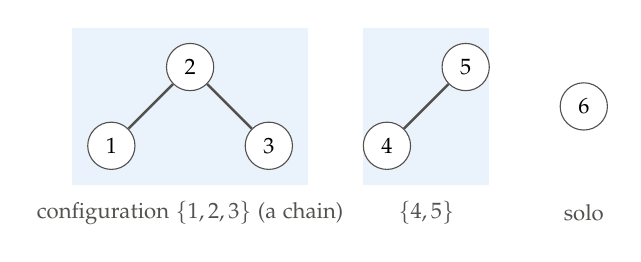
\begin{tikzpicture}[x=1cm,y=1cm, node/.style={circle, draw=ink, fill=white, minimum size=6mm, inner sep=0pt,
    font=\footnotesize}, edge/.style={ink, line width=0.9pt}]
  \fill[blueI!10] (-0.5,-0.5) rectangle (2.5,1.5);
  \fill[blueI!10] (3.2,-0.5) rectangle (4.8,1.5);
  \node[node] (a) at (0,0) {1}; \node[node] (b) at (1,1) {2}; \node[node] (c) at (2,0) {3};
  \node[node] (d) at (3.5,0) {4}; \node[node] (e) at (4.5,1) {5}; \node[node] (f) at (6,0.5) {6};
  \draw[edge] (a) -- (b) -- (c); \draw[edge] (d) -- (e);
  \node[font=\footnotesize, text=ink] at (1,-0.85) {configuration $\{1,2,3\}$ (a chain)};
  \node[font=\footnotesize, text=ink] at (4,-0.85) {$\{4,5\}$};
  \node[font=\footnotesize, text=ink] at (6,-0.85) {solo};
\end{tikzpicture}
\caption{The graph at one instant: three components, two of them configurations.}
\label{fig:graph}
\end{figure}

\begin{itemize}
  \item \textbf{Directed graph.} The edges carry an arrow. For the episodes the nodes are
        configurations, with an arrow $c\to c'$ when $c'$ starts as $c$ ends and they share a member.
        An episode is a connected component of this graph, arrows ignored.
  \item \textbf{Bipartite graph.} Nodes of two kinds, edges only between kinds. At one instant, the
        configurations ending and those starting, with an edge when they share a member. Each
        component is one event (Figure~\ref{fig:events}); its outcome follows from how many
        configurations it has on each side: one to one is a join or a leave (members added or
        removed), one to several a split, several to one a merge.
\end{itemize}

\begin{figure}[H]
\centering
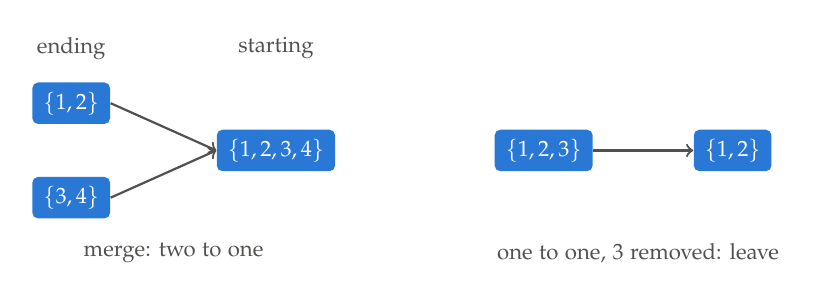
\begin{tikzpicture}[x=1cm,y=1cm, conf/.style={rounded corners=2pt, fill=blueI, text=white, font=\footnotesize,
    minimum height=5mm, inner xsep=4pt}, link/.style={->, ink, line width=0.8pt}]
  \node[conf] (c1) at (0,0.6) {$\{1,2\}$}; \node[conf] (c2) at (0,-0.6) {$\{3,4\}$};
  \node[conf] (c3) at (2.6,0) {$\{1,2,3,4\}$};
  \draw[link] (c1.east) -- (c3.west); \draw[link] (c2.east) -- (c3.west);
  \node[font=\footnotesize, text=ink] at (1.3,-1.3) {merge: two to one};
  \node[conf] (d1) at (6,0) {$\{1,2,3\}$};
  \node[conf] (d2) at (8.4,0) {$\{1,2\}$};
  \draw[link] (d1.east) -- (d2.west);
  \node[font=\footnotesize, text=ink] at (7.2,-1.3) {one to one, 3 removed: leave};
  \node[font=\footnotesize, text=ink] at (0,1.3) {ending}; \node[font=\footnotesize, text=ink] at (2.6,1.3) {starting};
\end{tikzpicture}
\caption{Two events: each is a connected component of the bipartite graph of the configurations
ending and starting at one instant.}
\label{fig:events}
\end{figure}

\textbf{Shape} (Section~\ref{sec:chains}). For a connected graph of $n$ nodes and $m$ edges:
\begin{itemize}
  \item \textbf{Density} $m/\binom{n}{2}$: the share of the node pairs joined by an edge.
  \item \textbf{Distance} between two nodes: the fewest edges of a path joining them. \textbf{Diameter}: the
        largest distance. In the chain 1--2--3 the diameter is 2; in a triangle, 1.
  \item \textbf{Complete graph}: every pair joined, density 1, diameter 1. \textbf{Tree}: $m=n-1$, the fewest
        edges that keep $n$ nodes connected, with no closed path; a \emph{chain} is a tree with diameter
        $n-1$, a \emph{star} one with diameter 2.
\end{itemize}

\textbf{Order} (Section~\ref{sec:leaders}). In a directed graph:
\begin{itemize}
  \item a \textbf{cycle} is a path that follows the arrows back to its start (A$\to$B$\to$C$\to$A);
        a graph with none is \textbf{acyclic}, and its nodes can be put in a line with every arrow
        pointing forward;
  \item a \textbf{source} has no arrow coming in: here, a pilot with nobody ahead, a leader;
  \item the \textbf{depth} of an acyclic graph is its longest chain of arrows: 1 for a star, $n-1$ for a line.
\end{itemize}
A directed triangle is \emph{transitive} (A$\to$B, B$\to$C, A$\to$C) or \emph{cyclic}; with arrows drawn
at random, 2 of its 8 orientations are cyclic.

\textbf{Configuration model} (Section~\ref{sec:partners}). A random graph with the \emph{degrees} (the number
of edges of each node) of a given one: each node gets as many half-edges as its degree, and the
half-edges are paired at random~\cite{newman2010}. It keeps how many partners each pilot had and
changes only who they were.

%======================================================================================
\section{Two models}\label{app:models}

\textbf{Ornstein--Uhlenbeck process}~\cite{uhlenbeck1930} (Section~\ref{sec:cohesion}). A quantity $\ell$
pulled back to 0 by a spring of rate $k$ and shaken by noise:
\begin{equation}
  d\ell=-k\,\ell\,dt+\sqrt{2k}\,\sigma\,dW .
\end{equation}
It forgets its value after $1/k$ and spreads by $\sigma$ around 0. Its mean square change after a lag
$s$ is $D(s)=\langle(\ell(t+s)-\ell(t))^2\rangle=2\sigma^2(1-e^{-ks})$: it grows as $2k\sigma^2 s$ at short
lags, like a free random walk, and stops at $2\sigma^2$ after $1/k$. With $k=0$ it is a random walk and
$D$ grows forever. A measurement noise of variance $c/2$ on each value adds $c$ to $D(s)$ at every lag.

\textbf{Birth--death chain} (Section~\ref{sec:fission}). A group of $n$ pilots gains one at rate $g(n)$ and
loses one at rate $l(n)$. Over a long time the transitions from $n$ to $n+1$ and back are equally
many, so the time spent at $n+1$ and at $n$, $T(n+1)$ and $T(n)$, satisfy $T(n)\,g(n)=T(n+1)\,l(n+1)$,
Eq.~\eqref{eq:chain}. Multiplying the ratios from 2 to $n$ gives $T(n)$. If every member joins others at
rate $a$ and leaves at rate $\mu$, $g(n)=an$, $l(n)=\mu n$ and $T(n)\propto x^n/n$ with $x=a/\mu$, the
log-series: the tail falls exponentially. A leaving rate that falls with $n$ makes it heavier.

%======================================================================================
\section{Phase at entry and exit}\label{app:phases}

\begin{table}[H]
\centering\footnotesize
\begin{tabular}{@{}l l l l@{}}
\toprule
 & climb (\%) & search (\%) & transition (\%) \\
\midrule
entering a group & 28.1 [27.6, 28.5] & 10.3 [10.0, 10.6] & 61.5 [61.0, 61.9] \\
leaving a group & 28.0 [27.6, 28.3] & 11.2 [10.9, 11.5] & 60.6 [60.1, 61.0] \\
share of time, alone & 29.1 [28.9, 29.3] & 10.1 [10.0, 10.2] & 60.8 [60.6, 61.0] \\
share of time, in a group & 33.0 [32.8, 33.2] & 9.4 [9.2, 9.6] & 57.6 [57.3, 57.9] \\
\bottomrule
\end{tabular}

\caption{Phase at the instant of entering or leaving a group, and shares of time in each phase
(percent, with 5--95\% bands; 1~Hz flights).}
\label{tab:phases}
\end{table}

%======================================================================================
\section{Reproducing the report}\label{app:reproduce}

From \texttt{analysis/groups/group-identification}, after the scripts of \emph{Group and solo flights}:
\begin{verbatim}
uv run python describe.py     # sizes, durations, events; about 15 s
uv run python cohesion.py     # delays and separations, one pass over every date; about 25 min
uv run python chains.py       # shapes and their H_loc; about 40 s
uv run python hierarchy.py    # order, switches, who leads; after cohesion.py
uv run python partners.py     # repeated partners; about 4 min
uv run python fission.py      # the birth-death chain; about 10 s
uv run python report/tables.py; uv run python report/structure_tables.py
cd report && latexmk -pdf group_structure.tex
\end{verbatim}
The per-date cache of \texttt{cohesion.py} is in \texttt{analyses/cohesion/all/days/} of the run on SSD\_DISANTE.


\end{document}
